\section{Multi-velocity binning, measured}
\label{app:multivel}

\subsection{Binned convolution}
\label{sec:multivel}

The single-velocity scope of Section~\ref{sec:fielddef} is extended by
splitting the velocity distribution into $B$ classes and running one
convolution per class; the near shell needs no binning, because each pair
carries its own velocity. The measurements below are on a $64^3$ grid of cell
$10^{-7}$\,m with $200$ sources of weight $5\times10^{-13}$\,C
($Q=-100$\,pC) on JURECA H100 (H100 \texttt{sm\_90}, CUDA 13.4).

\paragraph{Box representative.}
Each box is represented by its absolute-charge-weighted mean momentum, not by
the geometric box centre.  The mean minimises the angular and energy
deviations for which the error model charges the split, at no extra kernel
cost.  On a $200$-particle, $\gamma=10$, $5^\circ$ bunch the global L2 field
error against the $128$-box field falls from $13.2\%$ to $11.2\%$ at
$16$ boxes and from $4.31\%$ to $4.13\%$ at $64$ boxes.  The raw rows are in
\texttt{docs/measurements/velocity\_bin\_representative.csv}.

\paragraph{Single-velocity sanity.}
With zero spread the binned path is bitwise equal to the unbinned path:
$B=1$ and $B=16$ give bit-identical fields in all six components
($\max|\Delta|=0$).

\begin{table}[t]
\centering
\small
\caption{Binned multi-velocity peaks, $64^3$ grid of cell $10^{-7}$\,m,
$200$ sources of weight $5\times10^{-13}$\,C ($Q=-100$\,pC), $\gamma=10$.}
\label{tab:multivel}
\begin{tabular}{lrrrr}
\toprule
spread & $B\!=\!16$ $|B_z|$ (T) & $B\!=\!64$ $|B_z|$ (T) & $B\!=\!16$ $|B_y|$ (T) & $B\!=\!64$ $|B_y|$ (T) \\
\midrule
energy 5\%      & $2.32050\times10^{4}$ & $2.32049\times10^{4}$ & $0$ & $0$ \\
angular $5^\circ$ & $2.48202\times10^{4}$ & $2.48213\times10^{4}$ & $1.2948\times10^{3}$ & $1.2955\times10^{3}$ \\
\bottomrule
\end{tabular}
\end{table}

\begin{figure}[t]
\centering
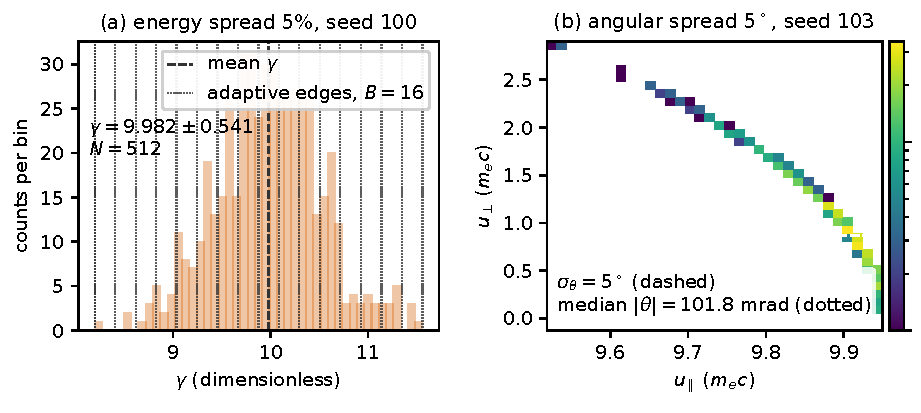
\includegraphics[width=0.98\linewidth]{figs/F_multivel_dist.pdf}
\caption{Sampled multi-velocity bunches ($\gamma=10$, 512 sources, seeds
100 and 103); the $B=16$ edges in (a) and the velocity boxes that produce
the field come from the same \texttt{VelocityBinning} per-axis min/max
path. (a) $\gamma$ histogram for the 5\% energy spread with the 16
adaptive edges drawn and the mean and standard deviation annotated;
(b) $u_\parallel$--$u_\perp$ density for the $5^\circ$ angular spread
with the nominal $5^\circ$ divergence and the measured median
$|\theta|=101.8$\,mrad marked; (c) relative deviation of the $B=16$ peaks
from the $B=64$ reference, $4.3\times10^{-6}$ (energy $B_z$),
$4.4\times10^{-5}$ (angular $B_z$) and $5.6\times10^{-4}$ (angular $B_y$),
with $B_y\equiv0$ for the energy case, so the field is
bin-independent at the stated $2.32050\times10^{4}$/$2.32049\times10^{4}$\,T
and $5.22\times10^{-2}$ ratio.}
\label{fig:multivel}
\end{figure}

Figure~\ref{fig:multivel} shows the sampled distributions and the
bin comparison. With a 5\% energy spread and $+y$ drift the $B_z$ peak is
$2.32050\times10^{4}$\,T at 16 bins and $2.32049\times10^{4}$\,T at 64
bins, $4.3\!\times\!10^{-4}\%$ apart ($4.3\!\times\!10^{-6}$ relative);
$B_y=0$ exactly, which is correct for a purely
longitudinal current. With a $5^\circ$ angular spread the $B_z$ peak moves
from $2.48202\times10^{4}$ to $2.48213\times10^{4}$\,T and $B_y$ from
$1294.8$ to $1295.5$\,T; the ratio $B_y/B_z$ is $5.22\times10^{-2}$, and
the two bin counts agree to $0.0043\%$ in $B_z$ and $0.056\%$ in $B_y$.
The tabulated angular peaks $2.48202\times10^{4}$ and
$2.48213\times10^{4}$\,T come from the pre-final code
(\texttt{c0bf82c}), whose host was not recorded.
On the final code the angular case gives $B_z=2.4663\times10^{4}$\,T,
$0.63\%$ below the tabulated $2.4820\times10^{4}$\,T, the velocity-binning
change in \texttt{VelocityBinning.cpp} between \texttt{c0bf82c} (table) and
\texttt{478f6e1} (final); the energy case reproduces to the printed
precision, $B_z=2.3205\times10^{4}$\,T.

\paragraph{1\,mrad case against the arbiter.}
The fluctuation bunch (Table~\ref{tab:configs} row ``1\,mrad, binned'':
$N=200$, weight $5\times10^{-13}$\,C each, $Q=-100$\,pC, $\gamma=10$,
$+y$ drift, 1.046\,mrad rms $x$-divergence) was re-run at 64 bins on the
$64^3$ grid of cell $10^{-7}$\,m and compared against the Gauss--Legendre
arbiter (unbinned, per-particle $u$, 698-node slice subset) as the
reference. On the x-y slice at $z=32$ cells ($z=3.2\,\si{\micro\metre}$,
the grid centre) picBunch gives
$B_y=7.835$\,T and $B_z=2.3336\times10^{4}$\,T, against arbiter values of
$7.759$\,T and $2.344\times10^{4}$\,T (factors $1.010\times$ and
$0.996\times$); on the z-y slice at $x=32$ cells ($x=3.2\,\si{\micro\metre}$)
the corresponding values are
$7.561$\,T / $7.519$\,T and $2.3159\times10^{4}$\,T /
$2.327\times10^{4}$\,T ($1.006\times$ and $0.995\times$). The 3-D $B_y$
peak is $8.734$\,T and $B_z$ is $2.3336\times10^{4}$\,T. The comparison
criterion is the per-component slice peaks---peak $|B_y|$ and peak $|B_z|$
on each plane---and the $B_y/B_z$ ratio; the worst deviation is $1.4\%$
(x-y ratio) and every per-component peak on every slice is within $1.0\%$.

Runtime: $B=64$, $64^3$, $200$ particles, \texttt{--near-shell fast}
($R=3$, tile 4, order 5), 248\,s, a legacy A30 value.

\section*{Far-tail switch validation}
\label{app:far-tail}

For the documented 20-cell, 4096-electron bunch (source radius $R=16.85$
cells, peak $45722.5$ V/m, tolerance level $45.72$ V/m), the quadrupole
margin of Eq.~\eqref{eq:tail} is $350$ cells, which exceeds the
$2^{28}$ padded-node cap, so the code falls back to the measured far-tail
switch. Table~\ref{tab:margin} gives the switch error: the worst
per-component $|\mathbf{E}_{\mathrm{tail}}-\mathbf{E}_{\mathrm{direct}}|$
against an independent direct charge sum in $13$ directions.

\begin{table}[t]
\centering
\small
\caption{Far-tail switch validation, 20-cell 4096-electron bunch,
$R=16.85$ cells, tolerance level $45.72$ V/m ($10^{-3}$ of the peak
$45722.5$ V/m). Worst per-component
$|\mathbf{E}_{\mathrm{tail}}-\mathbf{E}_{\mathrm{direct}}|$ against an
independent direct charge sum over $13$ directions. The switch at $6R$ is
the chosen switch: the error is $1.87\times10^{-3}$ of the tolerance level.
Legacy rosi\_v100 run: the direct-charge-sum comparison is not re-committed
in this repository, so these values are not re-measured here.}
\label{tab:margin}
\begin{tabular}{lrr}
\toprule
switch radius & worst err (V/m) & / tolerance level \\
\midrule
$2R$ ($33.7$ cells) & $4.80\times10^{1}$ & $1.05$ \\
$4R$ ($67.4$ cells) & $8.77\times10^{-1}$ & $1.92\times10^{-2}$ \\
$6R$ ($101.1$ cells) & $8.53\times10^{-2}$ & $1.87\times10^{-3}$ \\
$8R$ ($134.8$ cells) & $1.66\times10^{-2}$ & $3.63\times10^{-4}$ \\
\bottomrule
\end{tabular}
\end{table}

A $512^{3}$ output sampled outside the compute box confirms the
switch in practice: $36$ nodes including corners, worst
$|\mathbf{E}_{\mathrm{file}}-\mathbf{E}_{\mathrm{direct}}| = 2.8\times10^{-3}$
V/m against the $45.7$ V/m tolerance level ($6.1\times10^{-5}$ of it), and
every sample nonzero, i.e. no interior zero fill.
